% !TeX spellcheck = es_ES
%%% main.tex %%%

\documentclass[11pt]{article}
%%% style.tex %%%

%%%%% --------------------------------------------- %%%%%
%	   PACKAGES AND OTHER DOCUMENT CONFIGURATIONS       %
%%%%% --------------------------------------------- %%%%%


\usepackage{amsmath,amsfonts,stmaryrd,amssymb} % Math packages
\usepackage{fancyhdr}
\usepackage{enumerate} % Custom item numbers for enumerations
\usepackage[ruled]{algorithm2e} % Algorithms
\usepackage[framemethod=tikz]{mdframed} % Custom boxed/framed environments

\definecolor{codegray}{gray}{0.925}
\let\colortexttt\texttt
\renewcommand{\texttt}[1]{\colorbox{codegray}{\colortexttt{#1}}}

\setcounter{tocdepth}{2}

\usepackage{chngcntr}
\usepackage{tocloft}
\setlength{\cftfignumwidth}{3.5em}
\counterwithin{figure}{subsection}

\usepackage{xcolor} % Colours
\definecolor{mRed}{rgb}{0.8, 0, 0}
\definecolor{mGreen}{rgb}{0,0.6,0}
\definecolor{mGray}{rgb}{0.5,0.5,0.5}
\definecolor{mPurple}{rgb}{0.58,0,0.82}
\definecolor{mCyan}{RGB}{0, 183, 235}
\definecolor{mBlue}{rgb}{0.13,0.13,1}
\definecolor{backgroundColour}{rgb}{0.95,0.95,0.92}

\usepackage{caption}

\captionsetup{font=small}

\captionsetup{labelfont=bf, textfont=small}

\usepackage{listings} % File listings, with syntax highlighting
\lstset{
    aboveskip=12pt,
    belowskip=12pt,
	basicstyle=\ttfamily, % Typeset listings in monospace font
	extendedchars=true,  % Soporta caracteres extendidos
	literate={├}{{|-}}1 {─}{{-}}1 {●}{{$\bullet$}}1 {└}{{\texttt{\textbackslash}}}1
}

\lstdefinestyle{CppQtStyle}{
	backgroundcolor=\color{backgroundColour},
	commentstyle=\color{mGreen}\itshape,
	keywordstyle=\color{mCyan}\bfseries,           % C++ keywords
	keywordstyle=[2]\color{mViolet}\bfseries,      % Qt macros/signals/slots
	keywordstyle=[3]\color{mOrange},               % basic types
	numberstyle=\tiny\color{mGray},
	stringstyle=\color{mPurple},
	basicstyle=\fontfamily{pcr}\selectfont\footnotesize,
	breakatwhitespace=false,
	breaklines=true,
	captionpos=b,
	keepspaces=true,
	numbers=left,
	escapeinside={\%*}{*)},
	inputencoding=utf8,
	extendedchars=true,
	literate={á}{{\'a}}1 {ã}{{\~a}}1 {é}{{\'e}}1 {í}{{\'i}}1 {ó}{{\'o}}1 {ú}{{\'u}}1 {Á}{{\'A}}1 {É}{{\'E}}1 {Í}{{\'I}}1 {Ó}{{\'O}}1 {Ú}{{\'U}}1 {ñ}{{\~n}}1 {Ñ}{{\~N}}1,
	numbersep=5pt,
	showspaces=false,
	showstringspaces=false,
	showtabs=false,
	tabsize=2,
	language=C++,
	morekeywords={signals, slots, Q_OBJECT, emit},
	emph={main, connect, mapFromGlobal, setVisible, setDown}, % functions/methods to highlight
	emphstyle=\color{red}\bfseries
}

\lstdefinestyle{BashStyle}{
	backgroundcolor=\color{lightgray!10},
	keywordstyle=\color{blue!80!black}\bfseries,
	stringstyle=\color{red!70!black},
	basicstyle=\fontfamily{pcr}\selectfont\small,
	breakatwhitespace=false,
	breaklines=true,
	captionpos=b,
	keepspaces=true,
	numbers=none,
	showspaces=false,
	showstringspaces=false,
	showtabs=false,
	tabsize=2,
	language=bash,
	extendedchars=true,
	inputencoding=utf8
}

\lstdefinestyle{TextFileStyle}{
	backgroundcolor=\color{lightgray!5},
	basicstyle=\ttfamily\small,
	numbers=none,
	breaklines=true,
	captionpos=b,
	frame=single,
	rulecolor=\color{gray!30},
	showstringspaces=false,
	tabsize=2,
	language={}
}

\usepackage[most]{tcolorbox}

% src: https://xyquadrat.ch/blog/latex-boxes/
\tcbset {
	base/.style={
		arc=0mm,
		bottomtitle=0.5mm,
		boxrule=0mm,
		colbacktitle=black!10!white,
		coltitle=black,
		fonttitle=\bfseries,
		left=2.5mm,
		leftrule=1mm,
		right=3.5mm,
		title={#1},
		toptitle=0.75mm,
	}
}

\definecolor{brandblue}{rgb}{0.34, 0.7, 1}
\newtcolorbox{mainbox}[1]{
	colframe=brandblue,
	base={#1}
}

\newtcolorbox{subbox}[1]{
	colframe=black!30!white,
	base={#1}
}

\usepackage{colortbl} % Para \arrayrulecolor y colorear tablas
\usepackage{alltt}
\usepackage{array, multirow, tabularx, booktabs} % Tables
\usepackage{float}
\usepackage{tikz}
\usetikzlibrary{quotes,babel, positioning, shapes, shapes.geometric, arrows, calc, external, chains}
% \usetikzlibrary{arrows.meta, positioning, chains, positioning, shapes.geometric, shadows}
\usepackage{aeguill}
\usepackage{tikzpeople}
\usepackage{url}

\usepackage{pgfplots}

\usepackage[linktoc=none]{hyperref} % para enlaces. linktoc deshabilita indice
\hypersetup{
	colorlinks,
	linkcolor=blue,
	citecolor=blue,
	urlcolor={blue!80!black}, % urls
	pdftitle={Documentación QFotoPaint6},
	pdfsubject={InfGraf},
	pdfauthor={Hugo Sánchez Martínez}
}

\usepackage[spanish, es-nodecimaldot]{babel} % Paquete de español

\setlength{\arrayrulewidth}{1.5\arrayrulewidth} % Table rule thickness

% Cambiar título del ToC
\addto\captionsspanish{
	\renewcommand{\contentsname}
	{Contenidos}%
}

\usepackage{listingsutf8}    % Soporte para caracteres UTF-8
\usetikzlibrary{shadows,calc}

\usepackage[inline]{enumitem}
\makeatletter
% This command ignores the optional argument for itemize and enumerate lists
\newcommand{\inlineitem}[1][]{%
	\ifnum\enit@type=\tw@
	{\descriptionlabel{#1}}
	\hspace{\labelsep}%
	\else
	\ifnum\enit@type=\z@
	\refstepcounter{\@listctr}\fi
	\quad\@itemlabel\hspace{\labelsep}%
	\fi}
\makeatother

\renewcommand{\footnoterule}{%
	\vspace{1cm} % Espacio adicional antes de la línea
	\hrule width 0.8\textwidth % Ajusta el ancho de la línea (80% del ancho del texto)
	\vspace{2cm} % Espacio adicional después de la línea
}


%%%%% --------------------------------------------- %%%%%
%	                 DOCUMENT MARGINS
%%%%% --------------------------------------------- %%%%%

\usepackage{geometry} % Required for adjusting page dimensions and margins

\geometry{
	a4paper, % Papaer size
	margin={2cm,3cm},
	headheight=14pt, % Header height
	footskip=1cm, % Space from the bottom margin to the baseline of the footer
	headsep=1.2cm, % Space from the top margin to the baseline of the header
	%showframe, % Uncomment to show how the type block is set on the page
}

%%%%% --------------------------------------------- %%%%%
%	                      FONTS                         %
%%%%% --------------------------------------------- %%%%%

\usepackage[utf8]{inputenc} % Required for inputting international characters
\usepackage[T1]{fontenc} % Output font encoding for international characters
\usepackage[
protrusion=true,
activate={true,nocompatibility},
final,
tracking=true,
kerning=true,
spacing=true,
factor=1100]{microtype}
\SetTracking{encoding={*}, shape=sc}{40}


% Choose font:
\usepackage{mathptmx} 	 % Times
% \usepackage{mathpazo}  % Palatino
% \usepackage{lmodern}	 % Upgraded LaTeX font

%%%%% --------------------------------------------- %%%%%
%	            COMMAND LINE ENVIRONMENT                %
%%%%% --------------------------------------------- %%%%%

% Usage:
% \begin{commandline}
	%	\begin{verbatim}
		%		$ ls
		%
		%		Applications	Desktop	...
		%	\end{verbatim}
	% \end{commandline}

\mdfdefinestyle{commandline}{
	leftmargin=10pt,
	rightmargin=10pt,
	innerleftmargin=15pt,
	middlelinecolor=black!50!white,
	middlelinewidth=2pt,
	frametitlerule=false,
	backgroundcolor=black!5!white,
	frametitle={Bash},
	frametitlefont={\normalfont\sffamily\color{white}\hspace{-1em}},
	frametitlebackgroundcolor=black!50!white,
	nobreak,
}

% Define a custom environment for command-line snapshots
\newenvironment{commandline}{
	\medskip
	\begin{mdframed}[style=commandline]
	}{
	\end{mdframed}
	\medskip
}

%%%%% --------------------------------------------- %%%%%
%	             FILE CONTENTS ENVIRONMENT              %
%%%%% --------------------------------------------- %%%%%

% Usage:
% \begin{file}[optional filename, defaults to "File"]
	%	File contents, for example, with a listings environment
	% \end{file}

\mdfdefinestyle{file}{
	innertopmargin=1.6\baselineskip,
	innerbottommargin=0.8\baselineskip,
	innerleftmargin=1.6\baselineskip,
	topline=false, bottomline=false,
	leftline=false, rightline=false,
	leftmargin=2cm,
	rightmargin=2cm,
	singleextra={%
		\draw[fill=black!10!white](P)++(0,-1.2em)rectangle(P-|O);
		\node[anchor=north west]
		at(P-|O){\ttfamily\mdfilename};
		%
		\def\l{3em}
		\draw(O-|P)++(-\l,0)--++(\l,\l)--(P)--(P-|O)--(O)--cycle;
		\draw(O-|P)++(-\l,0)--++(0,\l)--++(\l,0);
	},
	nobreak,
}

% Define a custom environment for file contents
\newenvironment{file}[1][File]{ % Set the default filename to "File"
	\medskip
	\newcommand{\mdfilename}{#1}
	\begin{mdframed}[style=file]
	}{
	\end{mdframed}
	\medskip
}

%%%%% --------------------------------------------- %%%%%
%	          NUMBERED QUESTIONS ENVIRONMENT            %
%%%%% --------------------------------------------- %%%%%

% Usage:
% \begin{question}[optional title]
	%	Question contents
	% \end{question}

\mdfdefinestyle{question}{
	innertopmargin=1.2\baselineskip,
	innerbottommargin=0.8\baselineskip,
	roundcorner=5pt,
	nobreak,
	singleextra={%
		\draw(P-|O)node[xshift=1em,anchor=west,fill=white,draw,rounded corners=5pt]{%
			Question \theQuestion\questionTitle};
	},
}

\newcounter{Question} % Stores the current question number that gets iterated with each new question

% Define a custom environment for numbered questions
\newenvironment{question}[1][\unskip]{
	\bigskip
	\stepcounter{Question}
	\newcommand{\questionTitle}{~#1}
	\begin{mdframed}[style=question]
	}{
	\end{mdframed}
	\medskip
}


%%%%% --------------------------------------------- %%%%%
%	              WARNING TEXT ENVIRONMENT              %
%%%%% --------------------------------------------- %%%%%

% Usage:
% \begin{warn}[optional title, defaults to "Warning:"]
	%	Contents
	% \end{warn}

\mdfdefinestyle{warning}{
	topline=false, bottomline=false,
	leftline=false, rightline=false,
	nobreak,
	singleextra={%
		\draw(P-|O)++(-0.5em,0)node(tmp1){};
		\draw(P-|O)++(0.5em,0)node(tmp2){};
		\fill[black,rotate around={45:(P-|O)}](tmp1)rectangle(tmp2);
		\node at(P-|O){\color{white}\scriptsize\bf !};
		\draw[very thick](P-|O)++(0,-1em)--(O);%--(O-|P);
	}
}

% Define a custom environment for warning text
\newenvironment{warn}[1][Warning:]{ % Set the default warning to "Warning:"
	\medskip
	\begin{mdframed}[style=warning]
		\noindent{\textbf{#1}}
	}{
	\end{mdframed}
}


%%%%% --------------------------------------------- %%%%%
%                 INFORMATION ENVIRONMENT               %
%%%%% --------------------------------------------- %%%%%

% Usage:
% \begin{info}[optional title, defaults to "Info:"]
	% 	contents
	% 	\end{info}

\mdfdefinestyle{info}{%
	topline=false, bottomline=false,
	leftline=false, rightline=false,
	nobreak,
	singleextra={%
		\fill[black](P-|O)circle[radius=0.4em];
		\node at(P-|O){\color{white}\scriptsize\bf i};
		\draw[very thick](P-|O)++(0,-0.8em)--(O);%--(O-|P);
	}
}

% Define a custom environment for information
\newenvironment{info}[1][Info:]{ % Set the default title to "Info:"
	\medskip
	\begin{mdframed}[style=info]
		\noindent{\textbf{#1}}
	}{
	\end{mdframed}
}



\begin{document}

\title{
	\vspace{-5ex}
	\begin{figure}[H]
		\centering
		
\includegraphics[width=72mm]{figures/umu-logo}
	\end{figure}
	
	{\Large \textsc{Universidad de Murcia}}\\
	{\Large Facultad de Informática}\\ [12.5ex]
	{\Large \textsc{Prácticas de}\\ [1ex]}
	{\Huge Informática Gráfica}\\ [1ex]
	{\Large \textsc{4º de Grado en Ingeniería Informática}}\\
	{\Large \textsc{Profesor: Ginés García Mateos}} \\
	{\Large \textsc{Curso 2025/2026}} \\ 
	\vspace{10ex}
}

\author{
	{\Large Hugo Sánchez Martínez}\\[0.5ex]
	24450997L\\
	\texttt{hugo.s.m@um.es}\\
}

\pagestyle{fancy}
\fancyhf{}
\fancyhead[LE]{\nouppercase{\rightmark} \hfill \textbf{\nouppercase{\leftmark}}}   % Encabezado en la página izquierda (even) sin mayúsculas
\fancyhead[RO]{\nouppercase{\rightmark}}  % Encabezado en la página derecha (odd) sin mayúsculas
\setlength{\headheight}{25pt}  % Ajusta la altura del encabezado
\fancyfoot[R]{H. Sánchez}
\fancyfoot[C]{\thepage}

\date{\vspace{-10ex}}
\maketitle
\thispagestyle{empty} % Elimina el número de página de la portada
\clearpage

\thispagestyle{empty} % Elimina el número de página del ToC
\tableofcontents
\clearpage
\thispagestyle{empty} % Elimina el número de página del ToC
\listoffigures
\clearpage
\setcounter{page}{1}



\thispagestyle{empty}

\hrule
\vspace{-5.4ex}
\begin{abstract}
\vspace{1ex}
Este documento especifica la implementación de las prácticas de la asignatura de Informática Gráfica del último curso del grado en Ingeniería Informática de la Universidad de Murcia. \\

Dicha práctica consiste en el desarrollo de una aplicación de procesamiento multimedia, basada en herramientas y funcionalidades presentes en aplicaciones de edición de imágenes y vídeo ya existentes. El objetivo de este documento es describir en detalle el proceso de desarrollo de la aplicación, explicando las funcionalidades implementadas durante la práctica.
\vspace{0.5ex}
\end{abstract}
\hrule
\vspace{4ex}

\section{Introducción}

\textbf{QFotoPaint} es una aplicación de escritorio para el procesamiento de imágenes y vídeo desarrollada en C++, utilizando el \textit{framework} Qt y la librería OpenCV. \\

Inspirada en herramientas reales de edición como \textit{GIMP} o \textit{Photoshop}, QFotoPaint permite al usuario abrir, visualizar y editar múltiples imágenes simultáneamente, aplicando diferentes filtros, transformaciones y efectos de procesamiento digital de imagen de forma sencilla e intuitiva.

\section{Requisitos}

\noindent QFotoPaint requiere tener instalado un compilador compatible con el estándar C++17 o superior. \\

Es necesario disponer del entorno de desarrollo Qt Creator, junto con el framework Qt y la librería OpenCV, correctamente configurados para compilar y ejecutar la aplicación. \\

% TODO: mostrar como compilar desde \textit{source} usando qmake.

\section{Tecnologías}

\noindent Durante el desarrollo de QFotoPaint se han utilizado las siguientes tecnologías:

\begin{itemize}
	\item \textbf{Git}: Para el control de versiones y la gestión colaborativa del código fuente.
	\item \textbf{Qt Creator}: Entorno de desarrollo integrado (IDE) empleado para la codificación, depuración y diseño de la interfaz gráfica.
	\item \textbf{Qt Framework}: Biblioteca multiplataforma usada para la creación de la interfaz de usuario y la gestión de eventos.
	\item \textbf{OpenCV}: Librería de visión por computador utilizada para el procesamiento, filtrado y transformación de imágenes y vídeo.
	\item \textbf{qmake}: Herramienta de automatización utilizada para la configuración y compilación del proyecto Qt.
\end{itemize}

\clearpage

\section{Desarrollo}

\subsection{Información multimedia}

\noindent
Otra funcionalidad adicional es la de poder consultar información acerca de las imágenes abiertas. Datos como las dimensiones, el tipo o la relación de aspecto pueden ser útiles para el usuario. Para ello, es necesario crear una nueva clase, junto con un formulario, \texttt{InformacionMultimedia}.

\begin{info}[Observación]
	Se ha optado por representar todas las imágenes abiertas en lugar de únicamente la imagen seleccionada, debido a la simplicidad de la implementación, ya que basta con recorrer el arreglo de imágene \texttt{foto[]} de \texttt{struct ventana}.
\end{info}

\noindent
Para la función completa, consultar anexo. \\

% TODO: incluir en anexo

El diálogo diseñado ha sido inspirado en el utilizado por el programa VLC para consultar estadísticas e información acerca de los \textit{streams} de los ficheros multimedia:

\begin{figure}[H]
	\centering
	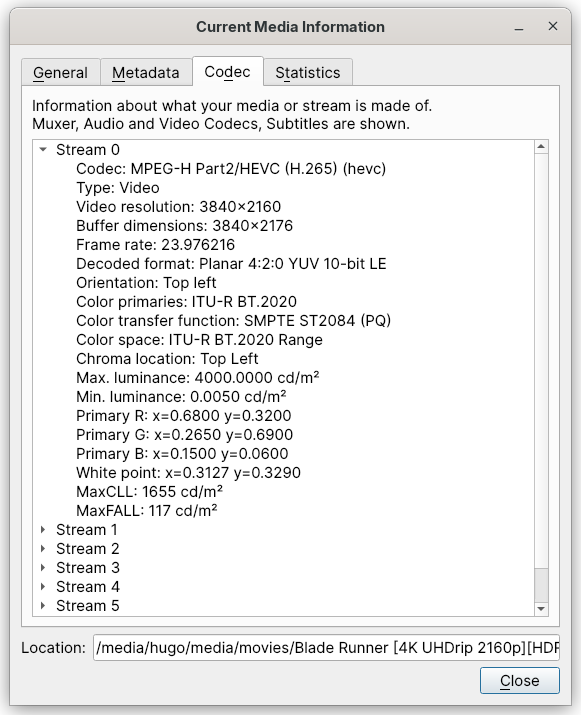
\includegraphics[width=0.4\textwidth]{figures/im_vlc}
	\caption{Diálogo de información multimedia en VLC.}
	\label{fig:im-vlc}
\end{figure}

El diseño se ha logrado usando un \texttt{QTabWidget} junto con un \texttt{QTreeWidget}. Para extender el contenido de éste al superior, se ha usado un \textit{layout} vertical. Esta implementación ofrece una gran comodidad a la hora añadir elementos a su nodo raíz en la clase \textit{src}.

\clearpage

\subsection{Ecualización del histograma}

\subsubsection{Introducción}

\noindent
La ecualización de histogramas es un método utilizado para mejorar el contraste de una imagen, al expandir las zonas que concentran mucho contraste. Su objetivo principal es transformar una imagen de entrada en otra imagen cuyo histograma tiene una distribución uniforme, aunque luego veremos que esto no es exactamente así, pues los histogramas no son completamente planos. \cite{opencv_histogram_equalization_tutorial} \\

La ecualización de histogramas no funciona igual en imágenes con un solo canal (imágenes de grises) que en imágenes a color. Para entender su funcionamiento, consideramos una imagen de grises \( X \), siendo \( n_i \) el número de ocurrencias para el nivel de grises \( i \). La probabilidad por tanto de que un píxel aleatorio tenga el valor de \( i \) es: 

\[ p_X (i) = \frac{n_i}{n}, \quad 0 \leq i < L \]

\noindent 
siendo \( L \) el número total de niveles de grises en la imagen. \( p_X (i)\) es el valor del histograma para \( i \). \\

\noindent
Definimos también la distribución acumulada de píxeles en \( X \) para el valor \( i \).


\[ \text{cdf}_X(i) = \sum_{j=0}^{i} p_X(j) \]

Para que esta función pueda emplearse como transformación de intensidades, debe normalizarse de manera 
que su valor máximo corresponda al nivel máximo de intensidad permitido (OpenCV usa 255). Es aquí donde empleamos el método que nos proporciona la librería de OpenCV \texttt{cv::equalizeHist}. \cite{opencv_equalizeHist_function}

\begin{mainbox}{\large equalizeHist()}
	\textbf{void cv::equalizeHist (InputArray src, OutputArray dst)}
	
	\vspace{2ex}
	
	Ecualiza el histograma de una imagen en escala de grises. \\
	La función ecualiza el histograma de la imagen de entrada utilizando el siguiente algoritmo:
	
	\begin{itemize}
		\item Calcular el histograma \(H\) para \texttt{src}.
		\item Normalizar el histograma de manera que la suma de los bins sea 255.
		\item Calcular el histograma acumulado:
		
		\[ H'_i = \sum_{0 \le j < i} H(j) \]
		
		\item Transformar la imagen utilizando \( H' \) como tabla de consulta:
		
		\[ \text{dst}(x,y) = H'(\text{src}(x,y)) \]
	\end{itemize}
	
	El algoritmo normaliza el brillo y aumenta el contraste de la imagen.
\end{mainbox}

\clearpage

\subsubsection{Implementación}

\noindent
El desarrollo de la ecualización del histograma está fuertemente basada en la del ajuste lineal
realizado en clase. Según la documentación, la funcionalidad debe permitir al usuario dos modos:

\begin{itemize}
	\item \textbf{Conjunto:} La operación se aplica de manera conjunta sobre un grupo completo de canales. Concretamente, se realizará sobre un conjunto específico (valor en HSV y luminancia en YCrCb). Es necesario convertir a uno de estos modos ya que, como se especifica en la teoría, pueden aparecer resultados erróneos si usamos el canal RGB, el cual mezcla el color con el brillo. \cite{wikipedia_hist_eq}
	
	\item \textbf{Independiente:} Si la imagen de entrada consta de varios canales, cada uno se procesa por separado sin tener en cuenta a los demás.
\end{itemize}

\noindent
Para implementar correctamente la funcionalidad, se ha optado por crear una nueva clase junto con un formulario, \texttt{EcualizacionHistograma}. El método implementado en \texttt{imagenes.cpp} es el siguiente:

\begin{lstlisting}[style=CppQtStyle, caption={Implementación de la ecualización del histograma}, label={lst:ecualhist}]
	// imagenes.cpp
	void ecualizacion_hist(int nfoto, int modo, bool guardar) {
	Mat img = foto[nfoto].img;
	Mat imres;
	
	if (img.channels() == 1) {  // imagen de grises
		equalizeHist(img, imres);
	} else if (modo == 0) {  // modo conjunto
		// convertir a HSV para separar luz del color
		Mat hsv;
		cvtColor(img, hsv, COLOR_BGR2HSV);
		
		vector<Mat> canales;
		split(hsv, canales);
		
		equalizeHist(canales[2], canales[2]);
		
		merge(canales, hsv);
		cvtColor(hsv, imres, COLOR_HSV2BGR);
	} else {  // modo independiente
		vector<Mat> canales;
		split(img, canales);
		
		for (size_t i = 0; i < 3; ++i)
		equalizeHist(canales[i], canales[i]);
		
		merge(canales, imres);
	}
	
	...
	
}
\end{lstlisting}

Como se puede ver en las líneas 10-16 del código \ref{lst:ecualhist}, se realiza una conversión de modelo a HSV para separar la luminosidad de la crominancia.

\section{Otras mejoras}

\subsection{Incremento del paso en arcoíris}

\noindent
Como propuesta del profesor, se ha diseñado una solución para que el usuario sea capaz de modificar el ``\textit{paso}'' con
el que se cambia de color del pincel en la herramienta ``Arcoíris''. Esta característica permitirá al usuario un mayor control 
sobre apariencia del efecto. \\

El ``paso'' se refiere a la velocidad de avance que en la secuencia de colores del espectro cada vez que se dibuja un píxel.  
Un paso pequeño provoca que los colores cambien lentamente, generando transiciones suaves y graduales entre tonos consecutivos.  
Por el contrario, un paso mayor acelera el cambio de color, produciendo un efecto más vivo. \\

Para implementar esta funcionalidad, se ha definido un nuevo elemento \texttt{QWidget} en \texttt{mainwindow.ui}. Este elemento
estará por defecto invisible, y su visibilidad cambiará al hacer \textit{click} sobre el botón de la herramienta. \\

También se ha valorado la necesidad de ocultar el panel si se pierde el foco en él. Se ha tenido que recurrir a un 
\textit{listener} de eventos de \texttt{QMouseEvent} ya que los paneles no proporcionan métodos \texttt{isHovered()}. 
Esta decisión es muy poco eficiente, pero aún así se ha decidido implementar. 

\begin{lstlisting}[style=CppQtStyle, caption={Mostrar/Ocultar panel al presionar la herramienta}]
	// mainwindow.cpp
	void MainWindow::on_toolButton_9_clicked() {
		herr_actual = HER_ARCOIRIS;
		ui->incrementoArcoirisWidget->setVisible(!ui->incrementoArcoirisWidget->isVisible());
	}

	...
	
	void MainWindow::mouseMoveEvent(QMouseEvent *event)	{
		if (ui->incrementoArcoirisWidget->isVisible()) {
			QPoint pos = event->pos();
			
			// Si el ratón no está dentro del widget y tampoco sobre el botón
			if (!ui->incrementoArcoirisWidget->geometry().contains(pos) &&
			!ui->toolButton_9->geometry().contains(pos)) {
				ui->incrementoArcoirisWidget->hide();
				ui->toolButton_9->setDown(false);
			}
		}
	}
\end{lstlisting}

En la clase \texttt{imagenes} también se han realizado algunas modificaciones. La primera es la necesidad de tener una
variable externa que se pueda utilizar en \texttt{mainwindow}, sustituyendo a la variable local \texttt{incremento}.

\begin{lstlisting}[style=CppQtStyle, caption={Mostrar/Ocultar según las coordenadas del ratón}]
	// imagenes.h
	constexpr int DEFAULT_INCREMENTO_ARCOIRIS = 10;
	extern int incremento_arcoiris;
\end{lstlisting}

\begin{lstlisting}[style=CppQtStyle, caption={Mostrar/Ocultar según las coordenadas del ratón}]
	// imagenes.cpp
	int incremento_arcoiris = DEFAULT_INCREMENTO_ARCOIRIS;
\end{lstlisting}

% TODO: Incluir modificacicones a MainWindow

%\begin{figure}[H]
%	\centering
%	\includegraphics[width=0.7\linewidth]{figures/}
%	\caption{}
%	\label{fig:}
%\end{figure}


\section{Bitácora}

\bibliographystyle{unsrt}
\bibliography{bibliography}


\end{document}